% !TeX root = ../main.tex
% !TEX root = ../main.tex
% -*- root: ../main.tex -*-
% -*- program: pdflatex -*-
\chapter{喷注味道鉴别流程}
基于机器学习算法设计喷注味道鉴别分类器需要有三个过程,即训练,验证和测试。训练阶段用一部分样本(训练集)对机器学习模型训练,使模型的鉴别能力不断优化提升;验证过程用一部分样本(验证集,不包含训练集)评估训练阶段获得模型的性能,并根据模型在验证集上的性能更改模型超参数,继续进行训练;测试过程用一部分样本(不能包含训练集,测试集)对经过训练,验证过程后的模型进行测试。整个系统主要由四部分组成:数据获取,数据预处理,特征选择和训练,其流程示意图如图~\ref{fig:model_process}~所示。
\begin{figure}[!htb]
  \centering
  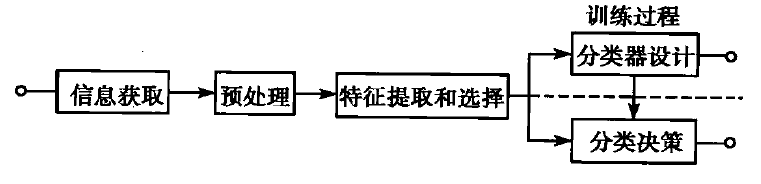
\includegraphics[width=10cm]{chap1/model_process.png}
  \caption{机器学习解决喷注味道鉴别问题流程}
  \label{fig:model_process}
\end{figure}
\section{原始数据获取}
现代高能物理实验通常利用大型探测装置对研究对象进行测量,实验得到的是探测装置对研究对象所记录的大量原始数据,它们包含了研究对象的模式信息~\cite{zhengzhipeng}。